% \documentclass[oneside]{report}
\documentclass[oneside,final,14pt,a4paper]{extreport}
% \documentclass[journal,onecolumn,a4paper,12pt]{IEEEtran}
% \usepackage[T2A]{fontenc}
\usepackage{listings}
\usepackage{subcaption}
\usepackage[demo]{graphicx}
\usepackage{fontspec}
\setmainfont{Times New Roman}



\usepackage{vmargin}
\setpapersize{A4}
\setmarginsrb{2.5cm}{2cm}{2cm}{2cm}{0pt}{10mm}{0pt}{13mm}
\usepackage{setspace}
\sloppy
\setstretch{1.5}
\usepackage{indentfirst}
\parindent=1.25cm

%%%%% ADDED TO SUPPORT TT BOLD FACES %%%%
\DeclareFontShape{OT1}{cmtt}{bx}{n}{<5><6><7><8><9><10><10.95><12><14.4><17.28><20.74><24.88>cmttb10}{}
\renewcommand{\ttdefault}{pcr}
%%%%% END %%%%%%%%%%%%%%%%%%%%%%%%%%%%%%% 
\usepackage{atbegshi,picture}
\AtBeginShipout{\AtBeginShipoutUpperLeft{%
  \put(\dimexpr\paperwidth-1cm\relax,-1.5cm){\makebox[0pt][r]{
\includegraphics[width=3cm]{figs/inno}}}%
}}


\usepackage[english]{babel}
\usepackage[backend=biber,style=ieee,autocite=inline]{biblatex}
\addbibresource{ref.bib}
\DefineBibliographyStrings{english}{%
  bibliography = {References},}
\usepackage{blindtext}
\usepackage{pdfpages}
\newenvironment{bottompar}{\par\vspace*{\fill}}{\clearpage}
\usepackage{amsmath,amsfonts}

\usepackage{amsthm}
\newtheorem{theorem}{Theorem}
\newtheorem{corollary}{Corollary}
\newtheorem{lemma}{Lemma}
\newtheorem{proposition}{Proposition}
\theoremstyle{definition}
\newtheorem{definition}{Definition}
\theoremstyle{remark}
\newtheorem*{remark}{Remark}
\theoremstyle{remark}
\newtheorem*{example}{Example}



\usepackage{float}
\usepackage{graphicx}
\graphicspath{{figs/}} %path to images
\usepackage{array}
\usepackage{multirow,array}
\usepackage{caption}
\usepackage{subcaption}
\usepackage{hyperref}
\usepackage{paralist}
\usepackage{listings}
\usepackage{zed-csp}
\usepackage{fancyhdr}
\usepackage{csquotes}
\usepackage{color}

\usepackage{upgreek} 
\usepackage{bm}
\usepackage{setspace}
\usepackage{booktabs}
\usepackage{longtable}
\usepackage[font=singlespacing, labelfont=bf]{caption}
\counterwithout{table}{chapter}
\renewcommand{\thetable}{\Roman{table}}
%Hints
\newcommand\pic[1]{(Fig. \ref{#1})} %Ref on figure
\newcommand\tab[1]{(Tab. \ref{#1})} %Ref on table


\usepackage{enumitem}
\newlist{inlinelist}{enumerate*}{1}
\setlist*[inlinelist,1]{%
  label=(\arabic*),
}




\pagestyle{fancyplain}

% remember section title
\renewcommand{\chaptermark}[1]%
	{\markboth{\chaptername~\thechapter~--~#1}{}}

% subsection number and title
\renewcommand{\sectionmark}[1]%
	{\markright{\thesection\ #1}}

\rhead[\fancyplain{}{\bf\leftmark}]%
      {\fancyplain{}{\bf\thepage}}
\lhead[\fancyplain{}{\bf\thepage}]%
      {\fancyplain{}{\bf\rightmark}}
\cfoot{} %bfseries


\newcommand{\dedication}[1]
   {\thispagestyle{empty}
     
   \begin{flushleft}\raggedleft #1\end{flushleft}
}

\begin{document}
% 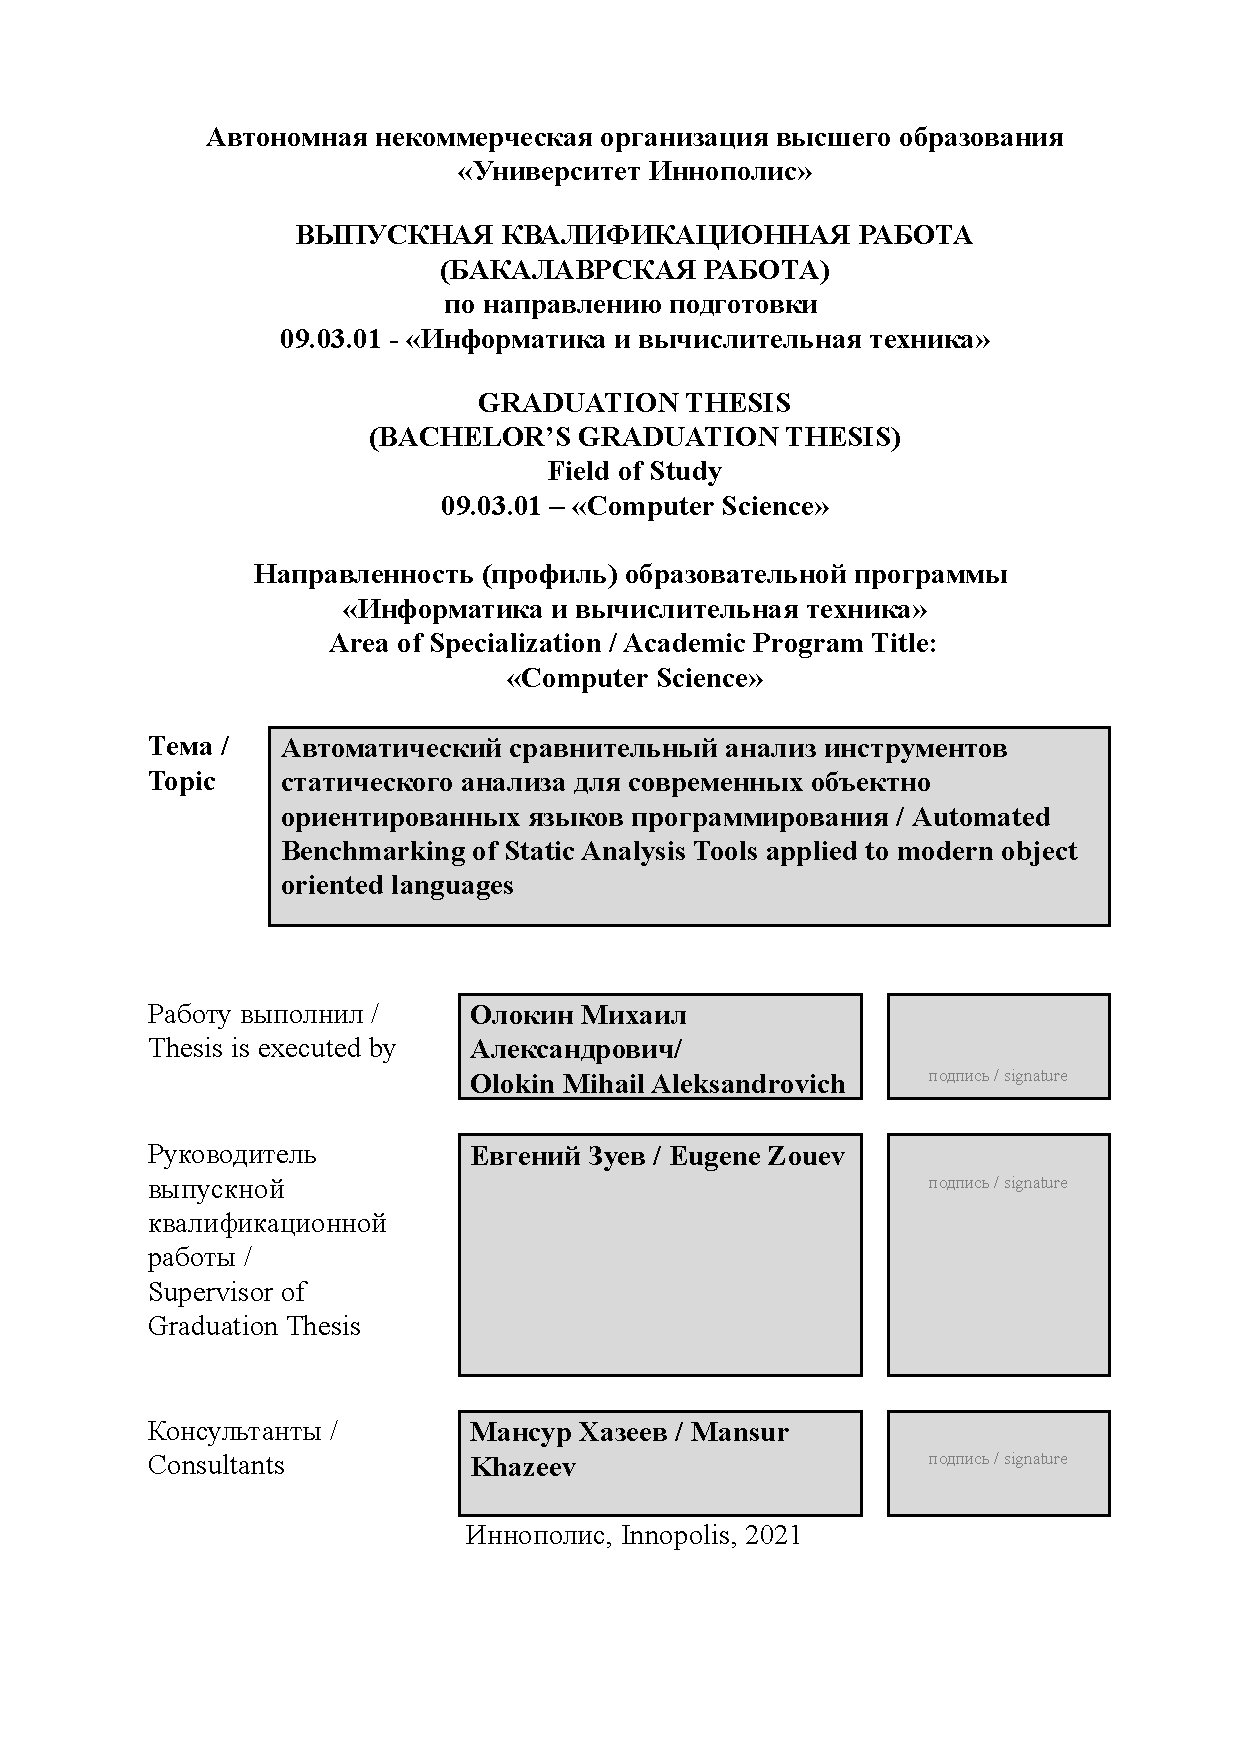
\includepdf[pages=-, offset={-\hoffset} {\voffset}]{title.pdf}
% \tableofcontents
% \listoftables
% \listoffigures



\newpage
\begin{abstract}

\end{abstract}

Depend on above part
\setcounter{page}{0}
\chapter{Introduction}
\label{chap:intro}
\chaptermark{Optional running chapter heading}



\label{sec:section}
Object-oriented programming languages have been adopted widely over the past two decades.
As of March 2022, the top five positions of the TIOBE index are occupied by Python, C, Java, C++ and C\#.
Four of these languages (with the exception of C) are considered object-oriented and, as the index suggests,
are widely adopted and used in large-scale commercial products.

\section{Properties of Object-Oriented Programming Languages}
According to \cite{oop1}, \textit{object-oriented} programming languages are the languages where the main unit of abstraction is an \textit{object}.
Objects encapsulate \textit{data}, which are the values of some type.
Some languages, e.g. Java and C++, distinguish between \textit{primitive types},
which represent low-level constructs like numbers or boolean values, and \textit{object types},
which represent a composite type. Objects may also contain operations on the said data,
known as \textit{methods}. Methods can take parameters and may return a value.

Objects should also obey certain definitive properties. As \cite{oop1} suggests, " the extent to which a particular language satisfies these properties defines how much of an object-oriented language it is." These properties are:
\begin{itemize}
    \item Encapsulation - an object should expose a well-defined interface through which it should be consumed.
          The irrelevant details of how an object implements this interface should be \textit{hidden} from the consumer.
    \item Inheritance - is a mechanism through which objects can share functionality and extend the behavior of other objects.
          Inheritance is a complex mechanism and its implementation differs from language to language.
          As per \cite{oop1}, "Inheritance enables programmers to reuse the definitions of previously defined structures.
          This clearly reduces the amount of work required in producing".
    \item Polymorphism - a possibility to define operations on objects in such a way,
          that they can accept and return values of multiple types.
    \item Dynamic (or late \cite{alankay}) binding - the implementation of the method to be run on an object is chosen at runtime. This implies that the implementation that is used during the runtime of a program may be \textit{different} from that of a type that is known statically (i.e. at compile time)

\end{itemize}

\section{Criticism}

Together with increasing adoption, OO programming techniques and languages have gained a substantial amount of valid criticism. Mansfield \cite{oopfailed} mentions most of these complaints, ultimately claiming that "...with OOP-inflected programming languages, computer software becomes more
verbose, less readable, less descriptive, and harder to modify and maintain". Many of these criticisms are being turned into recommendations, such as the famous "Design patterns: elements of reusable object-oriented software" \cite{GOFPatterns}. However, such recommendations are not the part of the language specification and thus can not be enforced by the language compiler. This leads to these recommendations often being misinterpreted or overused, especially by beginning software engineers.

\section{Analysis Tools}
To mitigate this complexity and enforce good practices, developers have created a lot of software tools. These tools can be divided into two categories: \textit{dynamic analyzers} and \textit{static analyzers}.

\textit{Dynamic analyzers} (also known as \textit{profilers}) inspect the state of the program as it is being executed. Dynamic analyzers collect important information about the program execution, such as CPU utilization and memory consumption and present it in the human-readable form. This information is crucial in applications where the performance plays an important role. Unfortunately, the tools require the program under analysis to be executed, which can be expensive or even impossible, e.g. when the program is to be run on dedicated hardware.

On the contrary, \textit{static analyzers} inspect the source code of the program (or one of its intermediate representations) \textit{without executing it} to locate common errors, anti-patterns and deviations from the accepted style conventions. Executing such tools isn't usually time-consuming or otherwise expensive, which is why they are a crucial part of continuous integration (CI) pipelines and integrated development environments (IDEs).
Despite being prone to false positives, static analysis tools can pinpoint the location of the error with greater precision.

Unlike dynamic analyzers, static analyzers operate on the source code, which allows them to inspect the program from a higher-level perspective. This means that static analyzers can improve the error reporting of programming language compilers, discover more problems, and  even automatically fix them.

Prior to analysis, many static analysis tools convert the source of the target language into some intermediate representation. This is done for several reasons. In general, this is done to extract the information from the source code that is relevant for analysis needs. Another common use case for employing an intermediate representation would be to
make the static analyzer work with more than one target language. In this case the representation serves as a common ground for the various analyzers. The examples of  intermediate representation are LLVM \cite{llvm} and Jimple \cite{vallee1998jimple} (used in SOOT \cite{vallee2010soot}).

\section{Research Objective}

In this thesis we present an implementation of a static analyzer for object-oriented programming languages with Elegant Objects \cite{eolang} (or EO) as an intermediate representation. This representation is based on $\phi$-calculus, a formal model that is designed to unify the varying semantics of object-oriented (OO) languages. It also claims to be a language with minimum verbosity, providing only the required subset of operators. The combination of a strict formal ground and a reduced feature set make EO a powerful intermediate representation for a static analyzer that should be able to capture many bugs specific to OO programs.

The rest of this thesis is structured as follows: Chapter 2 covers the existing work of finding bugs in OO programs, the semantics of EO and how it represents OO programs, Chapter 3 describes the implementation of the analyzer, Chapter 4 covers the evaluation of the analyzer, including testing and benchmarks and, finally, Chapter 5 concludes the thesis.

\chapter{Literature Review}
\label{chap:lr}
\chaptermark{Second Chapter Heading}
This chapter presents oveview of the theoretical concepts that the implementation relies on. Section \ref{lit:phicalc} briefly describes the relevant parts of $\varphi$-calculus: its syntax and semantics. Section \ref{lit:eo} explains how $\varphi$-calculus maps to EO, the intermediate representation the analyzers operate on. Section \ref{lit:encoding} shows how to encode basic object-oriented constructs (classes, methods, inheritance) by means of EO. 

\section{Methods \& Criteria}
The works surrounding $varphi$-calculus and EO appeared fairly recently and are largely not published. The works that are already published were provided by the supervisor. The preprints of the unpublished works were kindly provided by the authors. 

\section{$\varphi$-calculus}
\label{lit:phicalc}

EO is a programming language that implements $\varphi$-calculus, a formal model for object-oriented programming languages initially introduced by Bugayenko \cite{eolang}. In this thesis we use a refinement of $\varphi$-calculus proposed by Kudasov and Sim \cite{kudasov}.

\subsection{Objects and attributes}
At the heart of $\varphi$-calculus lies the concept of \textbf{object}.

\begin{definition}[Objects and attributes]
    An \textbf{object} is a set of pairs $\mkObject{n_0 \mapsto o_0, n_1 \mapsto o_1, \hdots, n_i \mapsto o_i, \hdots}$, where $n_i$ is a unique identifier and $o_i$ is an object. Such pairs are known as \textbf{attributes}. The first element is the \textbf{attribute name} the second element is the \textbf{attribute value}. An empty set $\mkObject{}$ is also a valid object. An attribute where the second element is $\mkObject{}$ is called \textbf{void} or \textbf{free}. Otherwise, it is known as \textbf{attached}.
\end{definition}

Attributes of object can be accessed by their names via the dot notation:
\begin{align*}
    \mkObject{x \mapsto y}.x \rightsquigarrow y
\end{align*}
In this case, this would reduce to just object $y$, which is defined elsewhere. $\rightsquigarrow$ means "is reduced to" or "evaluates to".

\subsection{Application}
Application can be used to create a new object where the values of the some or all free attributes are set. In other words, application can be used to create \textit{closed} objects from \textit{abstract} objects.

\begin{definition}[Abstract and closed objects]
    If an object has one or more free attributes it is called \textbf{abstract} or \textbf{open}. Otherwise, it is called \textbf{closed}.
\end{definition}

For example, object $a$ in \ref{lit:app} corresponds to a point in a two-dimensional space with coordinates $x = 1$, $y = 2$. The objects $1$ and $2$ can be defined in terms of $\varphi$-calculus, however the definition itself is out of the scope of this thesis.

\begin{align}
    point := \mkObject{x \mapsto \mkObject{}, y \mapsto \mkObject} \\
    \label{lit:app}
    a := point(x \mapsto 1, y \mapsto 2)                           \\
    a \rightsquigarrow \mkObject{x \mapsto 1, y \mapsto 2}
\end{align}


\subsection{Locators}

The revisision of $\varphi$-calculus by Kudasov and Sim \cite{kudasov} also defines special objects called \textbf{locators}, which are denoted as $\rho^i$, where $i \in \mathbb{N}$. Locators allow objects to reference other objects relatively to the object where the locator is used. For example, this can be used to (but is not limited to) encode definition of attributes in terms of other attributes of this object. Suppose there is an object $x$:
\begin{align*}
    x := \mkObject{a \mapsto \rho^0.b, b \mapsto c}
\end{align*}
The expression $x.a$ would be reduced to the value of object $c$. This happens because $x.a$ references $x.b$ via $\rho^0$, which means the immediate enclosing object. In more complicated examples, like \ref{lit:complex}.

\begin{align}
    \label{lit:complex}
    x := \mkObject{a \mapsto \mkObject{c \mapsto \rho^1.b}, b \mapsto d} \\
    x.a.c \rightsquigarrow d
\end{align}

$\rho$ can be used to define attributes of inner objects in terms of attributes of outer objects, or even outer objects themselves.

\subsection{$\varphi$-attribute}
Objects can define a special attribute with name $\varphi$. This attribute redirects attribute access to its value when the enclosing object does not have an attribute with such a name (fig. \ref{lit:phi}).

\begin{align}
    \label{lit:phi}
    a := \mkObject{d \mapsto y}                    \\
    \label{lit:decorated}
    x := \mkObject{\varphi \mapsto a, c \mapsto g} \\
    x.d \rightsquigarrow x.\varphi.d \rightsquigarrow y
\end{align}

If the attribute is present both in the object and its $\varphi$-attribute, the attribute in the object takes precedence:
\begin{align*}
    a := \mkObject{d \mapsto y}                             \\
    x := \mkObject{\varphi \mapsto a, \textbf{d} \mapsto g} \\
    x.d \rightsquigarrow g
\end{align*}

In \ref{lit:decorated}, Bugayenko \cite{eolang} refers to object $a$ as \textbf{decorated object}, where the "decorated" part refers to the decorator pattern described in \cite[Chapter 4]{GOFPatterns}. This technique of extending an object is also known as \textit{delegation} \cite{raiha_delegation:_1994} in object-oriented languages.

\subsection{A complex example}
Tying everything together, figure \ref{fig:fibo} shows how $\varphi$-calculus can be used to compute Fibonacci numbers.

% fib ->
%   [ n -> ?
%   , @ -> n.less(_1 -> 2).if(
%       _1 -> n
%     )(
%       _2 -> fib(n -> n.sub(_1 -> 1)).add(_1 -> fib(n -> n.sub(_1 -> 2)))
%     )
%   ]
% ].fib(n -> 7)
\begin{figure}
    \begin{align*}
        fib := &\mkObject{                                    \\
            n &\mapsto \mkObject{},                           \\
            \varphi &\mapsto \rho^0.n.less(n \mapsto 2).if( \\
            &ifTrue \mapsto n,                                \\
            &ifFalse \mapsto                                  \\
            &fib(n \mapsto \rho^0.n.sub(n \mapsto 1))\\
            &.add(n \mapsto fib(n \mapsto \rho^0.n.sub(n \mapsto2)\\)\\)\\)\\
        }
    \end{align*}
    \caption{Fibonacci numbers in $\varphi$-calculus}
    \label{fig:fibo}
\end{figure}

% \subsection{Dataization}
% $\varphi$-attribute plays an important role in the process of \textit{dataization}, which is a term coined by Bugayenko in \cite{eolang} that describes the evaluation of an EO program.

\section{EO}
\label{lit:eo}
EOLANG, or simply EO, is a programming language created by Bugayenko \cite{eolang} which is a direct implementation of $\varphi$-calculus with some extensions. However, their implementation contains features that are irrelevant to the scope of this thesis. Moreover, there is a notable difference between Bugayenko version of EO and $\phi$-calculus by \cite{kudasov} in the definition of locators (or "parent objects"). In the work by Bugayenko locators are \textit{attributes}, whereas in \cite{kudasov} they are \textit{objects}. In this thesis, similarly to the $\varphi$-calculus, we are going to use a different version of EO which is a direct translation of the calculus defined in \ref{lit:phicalc}. The table of translation is shown in figure \ref{fig:phitoeo}.

\begin{figure}
    \begin{center}
        \begin{tabular}{|c|c|c|}
            \hline
                                & $\varphi$-calculus         & EO \\
            \hline
            Objects             & $obj := \mkObject{a \mapsto x, b \mapsto y}$ &  \lstinputlisting{code/objects.eo}\\
            \hline
            Free Attrubutes     &   $point := \mkObject{x \mapsto \mkObject{}, y \mapsto \mkObject}$   &  \lstinputlisting{code/free_attributes.eo}   \\
            \hline
            Application &     $a := point(x \mapsto 1, y \mapsto 2)$ & \lstinputlisting{code/application.eo} \\
            \hline
            $\varphi$-attribute & $x := \mkObject{\varphi \mapsto a, c \mapsto g}$ & \lstinputlisting{code/phi_attribute.eo}   \\
            \hline
            Fibonacci example & Fig. \ref{fig:fibo} & \lstinputlisting{code/fibonacci.eo}   \\
            \hline
            $\rho^0$ & $\rho^0$ &  \$ \\
            \hline
            $\rho^1$ & $\rho^1$ &  \textasciicircum \\
            \hline
            $\rho^3$ & $\rho^3$ &  \textasciicircum.\textasciicircum.\textasciicircum \\
            \hline
        \end{tabular}
    \end{center}
    \caption{Mapping $\varphi$-calculus to EO}
    \label{fig:phitoeo}
\end{figure}

\section{Describing object-oriented programs with EO}
\label{lit:encoding}
Before analyzing programs written in object-oriented programming languages, it is necessary to translate them into EO while preserving the semantics of the original language. This section presents a simplified version of such an encoding that is assumed by analyzers described in this thesis. The encoding was largely insipired by \cite{bugayenko_reducing_2021} with some changes aimed mostly at simplifying the analysis process.

\subsection{Classes}
Classes are modelled as closed EO objects. Class-level (i.e. "static") attributes become attributes of the class object. Constructor is represented by an attribute-object "new" of the class object. This object may take parameters to produce an instance of the object.

All instance attributes and methods are defined inside the object returned by the "new" object. Inheritance is modelled as decoration in EO. Class instances (a.k.a objects in Java) are created
by applying the "new" object to the required parameters.

\subsection{Methods}
Methods are modelled as EO objects, similarly to classes. These objects can take parameters.
Instance methods are required to accept a special \textbf{self} attribute in addition to other parameters. This parameter is used to pass an instance of the object calling the method (hence the name - "self").
"self" parameter can be used to call instance methods inside other instance methods. The call to the method takes the following form:
\begin{lstlisting}
    self.method_name self arg1 arg2, etc.
\end{lstlisting}

The return value of the method is represented by the value of the $\varphi$ attribute ("@" symbol in EO). In order to call the instance method we need to instantiate the object first. Then we can call the method by accessing the instance's attribute with the method name and passing the instance object to it as the first argument.

\subsection{Examples of translation}
The examples of such translation applied to simple Java programs can be found in the subsequent sections, namely figures \ref{fig:mutualrec_basic} and \ref{fig:unjustified_before}.
\section{Fragile Base Class Problem}

\subsection{Unanticipated Mutual Recursion}
Unanticipated mutual recursion is a problem that occurs as a result of unconstrained inheritance. Suppose we have an object named Base with two methods - $f$ and $g$. Method $g$ calls method $f$, whereas $f$ does not.


Then, there is a class called Derived that extends Base and redefines the method $f$ in a way that it calls $g$. When we call a method $f$ on an instance of Derived, we get a stack overflow error: method $f$ calls method $g$, method $g$ calls method $f$ and so on \pic{fig:mutualrec_basic}.

It is important to note that we are not interested in detecting mutual recursion between the two methods of the same class. We are only interested the cases where mutual recursion occurs as a result of redefining one of the methods of the superclass. The example \pic{fig:oddeven} shows the class with two mutually-recursive methods \textit{isOdd} and \textit{isEven}. In this case the recursion is anticipated and necessary, so it is not a defect.

\begin{figure}
    \centering
    \begin{subfigure}{0.4\textwidth}
        \lstinputlisting[language=Java]{code/mutualrec.java}
        \caption{Java}
    \end{subfigure}
    \hfill
    \begin{subfigure}{0.4\textwidth}
        \lstinputlisting{code/mutualrec.eo}
        \caption{EO}
    \end{subfigure}
    \caption{Example of unanticipated mutual recursion}
    \label{fig:mutualrec_basic}
\end{figure}

\begin{figure}
    \centering
    \begin{subfigure}{0.4\textwidth}
        \lstinputlisting[language=Java]{code/NumericOps.java}
        \caption{Java}
    \end{subfigure}
    \hfill
    \begin{subfigure}{0.4\textwidth}
        \lstinputlisting{code/numeric_ops.eo}
        \caption{EO}
    \end{subfigure}
    \caption{Example without unanticipated mutual recursion.}
    \label{fig:oddeven}
\end{figure}

\subsection{Unjustified Assumption in Subclass}
This defect \cite[Section 3.3]{fragilebaseclass} occurs when the superclass is refactored by \textit{inlining} the calls to the method that can be redefined by the subclass. The term inlining refers to replacing the method call with its body. Consider an example \pic{fig:unjustified_before}. Class $M$ extends class $C$, redefining method $l$ to weaken its precondition. Consequently, the precondition in method $m$ of class $M$ is also weakened, because it relies on calling the method $l$.

Now, suppose that class $C$ comes from some external library, and class $M$ is defined in the user code. Library maintainer decides to refactor class $C$ by inlining the call to $l$ in method $m$ \pic{fig:unjustified_after}. Observe what happens to the class $M$. Now that $m$ in class base has an assert, the redefinition of method $n$ in class $M$ has its precondition strengthened as compared to its version in class $C$. Therefore, the seemingly safe refactoring in base class broke the invariants in the subclasses. The name of the defect come from the fact that the subclasses usually $M$ \textit{assume} that the method $m$ should be implemented in terms of method $l$. The examples in fig. \ref{fig:unjustified_before} and \ref{fig:unjustified_after} show that such an assumption is indeed not justified, and the maintainers of class $C$ can change it as they deem fit.

\begin{figure}
    \centering
    \begin{subfigure}{0.4\textwidth}
        \lstinputlisting[language=Java]{code/Unjustified.java}
        \caption{Java}
    \end{subfigure}
    \hfill
    \begin{subfigure}{0.4\textwidth}
        \lstinputlisting{code/unjustified.eo}
        \caption{EO}
    \end{subfigure}
    \caption{Example of unjustified assumption in subclass (before revision)}
    \label{fig:unjustified_before}
\end{figure}

\begin{figure}
    \centering
    \begin{subfigure}{0.4\textwidth}
        \lstinputlisting[language=Java]{code/UnjustifiedRevised.java}
        \caption{Java}
    \end{subfigure}
    \hfill
    \begin{subfigure}{0.4\textwidth}
        \lstinputlisting{code/unjustified_revised.eo}
        \caption{EO}
    \end{subfigure}
    \caption{Example of unjustified assumption in subclass (after revision)}
    \label{fig:unjustified_after}
\end{figure}



\newpage

% \chapter{Overview of EO}
\chapter{Methodology}
\label{chap:met}
This chapter presents the formal basis required to understand the implementation part. Section \ref{met:phicalc} briefly describes the relevant parts of $\varphi$-calculus: its syntax and semantics. Section \ref{met:eo} explains how $\varphi$-calculus maps to EO, the intermediate representation the analyzers operate on. Section \ref{met:encoding} shows how to encode basic object-oriented constructs (classes, methods, inheritance) by means of EO. Sections \ref{met:mutualrec} and \ref{met:unjustified} explain their respective defect type and how it can be detected in an EO program.

\section{$\varphi$-calculus}
\label{met:phicalc}

EO is a programming language that implements $\varphi$-calculus, a formal model for object-oriented programming languages initially introduced by Bugayenko \cite{eolang}. In this thesis we use a refinement of $\varphi$-calculus proposed by Kudasov and Sim \cite{kudasov}.

\subsection{Objects and attributes}
At the heart of $\varphi$-calculus lies the concept of \textbf{object}.

\begin{definition}[Objects and attributes]
    An \textbf{object} is a set of pairs $\mkObject{n_0 \mapsto o_0, n_1 \mapsto o_1, \hdots, n_i \mapsto o_i, \hdots}$, where $n_i$ is a unique identifier and $o_i$ is an object. Such pairs are known as \textbf{attributes}. The first element is the \textbf{attribute name} the second element is the \textbf{attribute value}. An empty set $\mkObject{}$ is also a valid object. An attribute where the second element is $\mkObject{}$ is called \textbf{void} or \textbf{free}. Otherwise, it is known as \textbf{attached}.
\end{definition}

Attributes of object can be accessed by their names via the dot notation:
\begin{align*}
    \mkObject{x \mapsto y}.x \rightsquigarrow y
\end{align*}
In this case, this would reduce to just object $y$, which is defined elsewhere. $\rightsquigarrow$ means "is reduced to" or "evaluates to".

\subsection{Application}
Application can be used to create a new object where the values of the some or all free attributes are set. In other words, application can be used to create \textit{closed} objects from \textit{abstract} objects.

\begin{definition}[Abstract and closed objects]
    If an object has one or more free attributes it is called \textbf{abstract} or \textbf{open}. Otherwise, it is called \textbf{closed}.
\end{definition}

For example, object $a$ in \ref{met:app} corresponds to a point in a two-dimensional space with coordinates $x = 1$, $y = 2$. The objects $1$ and $2$ can be defined in terms of $\varphi$-calculus, however the definition itself is out of the scope of this thesis.

\begin{align}
    point := \mkObject{x \mapsto \mkObject{}, y \mapsto \mkObject} \\
    \label{met:app}
    a := point(x \mapsto 1, y \mapsto 2)                           \\
    a \rightsquigarrow \mkObject{x \mapsto 1, y \mapsto 2}
\end{align}


\subsection{Locators}

The revisision of $\varphi$-calculus by Kudasov and Sim \cite{kudasov} also defines special objects called \textbf{locators}, which are denoted as $\rho^i$, where $i \in \mathbb{N}$. Locators allow objects to reference other objects relatively to the object where the locator is used. For example, this can be used to (but is not limited to) encode definition of attributes in terms of other attributes of this object. Suppose there is an object $x$:
\begin{align*}
    x := \mkObject{a \mapsto \rho^0.b, b \mapsto c}
\end{align*}
The expression $x.a$ would be reduced to the value of object $c$. This happens because $x.a$ references $x.b$ via $\rho^0$, which means the immediate enclosing object. In more complicated examples, like \ref{met:complex}.

\begin{align}
    \label{met:complex}
    x := \mkObject{a \mapsto \mkObject{c \mapsto \rho^1.b}, b \mapsto d} \\
    x.a.c \rightsquigarrow d
\end{align}

$\rho$ can be used to define attributes of inner objects in terms of attributes of outer objects, or even outer objects themselves.

\subsection{$\varphi$-attribute}
Objects can define a special attribute with name $\varphi$. This attribute redirects attribute access to its value when the enclosing object does not have an attribute with such a name (fig. \ref{met:phi}).

\begin{align}
    \label{met:phi}
    a := \mkObject{d \mapsto y}                    \\
    \label{met:decorated}
    x := \mkObject{\varphi \mapsto a, c \mapsto g} \\
    x.d \rightsquigarrow x.\varphi.d \rightsquigarrow y
\end{align}

If the attribute is present both in the object and its $\varphi$-attribute, the attribute in the object takes precedence:
\begin{align*}
    a := \mkObject{d \mapsto y}                             \\
    x := \mkObject{\varphi \mapsto a, \textbf{d} \mapsto g} \\
    x.d \rightsquigarrow g
\end{align*}

In \ref{met:decorated}, Bugayenko \cite{eolang} refers to object $a$ as \textbf{decorated object}, where the "decorated" part refers to the decorator pattern described in \cite[Chapter 4]{GOFPatterns}. This technique of extending an object is also known as \textit{delegation} \cite{raiha_delegation:_1994} in object-oriented languages.

\subsection{Complete example}
Tying everything together, figure \ref{fig:fibo} shows how $\varphi$-calculus can be used to compute Fibonacci numbers.

% fib ->
%   [ n -> ?
%   , @ -> n.less(_1 -> 2).if(
%       _1 -> n
%     )(
%       _2 -> fib(n -> n.sub(_1 -> 1)).add(_1 -> fib(n -> n.sub(_1 -> 2)))
%     )
%   ]
% ].fib(n -> 7)
\begin{figure}
    \begin{align*}
        fib := &\mkObject{                                    \\
            n &\mapsto \mkObject{},                           \\
            \varphi &\mapsto \rho^0.n.less(n \mapsto 2).if( \\
            &ifTrue \mapsto n,                                \\
            &ifFalse \mapsto                                  \\
            &fib(n \mapsto \rho^0.n.sub(n \mapsto 1))\\
            &.add(n \mapsto fib(n \mapsto \rho^0.n.sub(n \mapsto2)\\)\\)\\)\\
        }
    \end{align*}
    \caption{Fibonacci numbers in $\varphi$-calculus}
    \label{fig:fibo}
\end{figure}

% \subsection{Dataization}
% $\varphi$-attribute plays an important role in the process of \textit{dataization}, which is a term coined by Bugayenko in \cite{eolang} that describes the evaluation of an EO program.

\section{EO}
\label{met:eo}
EOLANG, or simply EO, is a programming language created by Bugayenko \cite{eolang} which is a direct implementation of $\varphi$-calculus with some extensions. However, their implementation contains features that are irrelevant to the scope of this thesis. Moreover, there is a notable difference between Bugayenko version of EO and $\phi$-calculus by \cite{kudasov} in the definition of locators (or "parent objects"). In the work by Bugayenko locators are \textit{attributes}, whereas in \cite{kudasov} they are \textit{objects}. Consequently, in this thesis, similarly to the $\varphi$-calculus, we are going to use a different version of EO which is a direct translation of the calculus defined in \ref{met:phicalc}. The table of translation is shown in figure \ref{fig:phitoeo}.

\begin{figure}
    \begin{center}
        \begin{tabular}{|c|c|c|}
            \hline
                                & $\varphi$-calculus         & EO \\
            \hline
            Objects             & $obj := \mkObject{a \mapsto x, b \mapsto y}$ &  \lstinputlisting{code/objects.eo}\\
            \hline
            Free Attrubutes     &   $point := \mkObject{x \mapsto \mkObject{}, y \mapsto \mkObject}$   &  \lstinputlisting{code/free_attributes.eo}   \\
            \hline
            Application &     $a := point(x \mapsto 1, y \mapsto 2)$ & \lstinputlisting{code/application.eo} \\
            \hline
            $\varphi$-attribute & $x := \mkObject{\varphi \mapsto a, c \mapsto g}$ & \lstinputlisting{code/phi_attribute.eo}   \\
            \hline
            Fibonacci example & Fig. \ref{fig:fibo} & \lstinputlisting{code/fibonacci.eo}   \\
            \hline
            $\rho^0$ & $\rho^0$ &  \$ \\
            \hline
            $\rho^1$ & $\rho^1$ &  \textasciicircum \\
            \hline
            $\rho^3$ & $\rho^3$ &  \textasciicircum.\textasciicircum.\textasciicircum \\
            \hline
        \end{tabular}
    \end{center}
    \caption{Mapping $\varphi$-calculus to EO}
    \label{fig:phitoeo}
\end{figure}

\section{Describing object-oriented programs with EO}
\label{met:encoding}
Before analyzing programs written in object-oriented programming languages, it is necessary to translate them into EO while preserving the semantics of the original language. This chapter presents a simplified version of such an encoding that is assumed by analyzers described in this thesis.

\subsection{Classes}
Classes are modelled as closed EO objects. Class-level (i.e. "static") attributes become attributes of the class object. Constructor is represented by an attribute-object "new" of the class object. This object may take parameters to produce an instance of the object.

All instance attributes and methods are defined inside the object returned by the "new" object. Inheritance is modelled as decoration in EO. So, a full example of EO translation would look like this. Class instances (a.k.a objects in Java) are created
by applying the "new" object to the required parameters.

\subsection{Methods}
Methods are modelled as EO objects, similarly to classes. These objects can take parameters.
Instance methods are required to accept a special "self" attribute in addition to other parameters. This parameter is used to pass an instance of the object calling the method (hence the name - "self").
"self" parameter can be used to call instance methods inside other instance methods.

The return value of the method is represented by the value of the $\varphi$ attribute ("@" symbol in EO). In order to call the instance method we need to instantiate the object first. Then we can call the method by accessing the instance's attribute with the method name and passing the instance object to it as the first argument.

\section{Detecting Unanticipated Mutual Recursion}
\label{met:mutualrec}
\subsection{Problem Statement}
Unanticipated mutual recursion is a problem that occurs as a result of unconstrained inheritance. Suppose we have an object named Base with two methods - $f$ and $g$. Method $g$ calls method $f$, whereas $f$ does not.


Then, there is a class called Derived that extends Base and redefines the method $f$ in a way that it calls $g$. When we call a method $f$ on an instance of Derived, we get a stack overflow error: method $f$ calls method $g$, method $g$ calls method $f$ and so on (figure \ref{fig:mutualrec_basic}).

It is important to note that we are not interested in detecting mutual recursion between the two methods of the same class. We are only interested the cases where mutual recursion occurs as a result of redefining one of the methods of the superclass. The example in fig. \ref{fig:oddeven} shows the class with two mutually-recursive methods "isOdd" and "isEven". In this case the recursion is anticipated and necessary, so it is not a defect.

\begin{figure}
    \centering
    \begin{subfigure}{0.4\textwidth}
        \lstinputlisting[language=Java]{code/mutualrec.java}
        \caption{Java}
    \end{subfigure}
    \hfill
    \begin{subfigure}{0.4\textwidth}
        \lstinputlisting{code/mutualrec.eo}
        \caption{EO}
    \end{subfigure}
    \caption{Example of unanticipated mutual recursion}
    \label{fig:mutualrec_basic}
\end{figure}

\begin{figure}
    \centering
    \begin{subfigure}{0.4\textwidth}
        \lstinputlisting[language=Java]{code/NumericOps.java}
        \caption{Java}
    \end{subfigure}
    \hfill
    \begin{subfigure}{0.4\textwidth}
        \lstinputlisting{code/numeric_ops.eo}
        \caption{EO}
    \end{subfigure}
    \caption{Example without unanticipated mutual recursion.}
    \label{fig:oddeven}
\end{figure}

\subsection{Proposed solution}
The solution to the problem lies in detecting the cycles in the call-graphs of all the objects. For each class-object in the program, do the following:
\begin{enumerate}
    \item Detect the decorated class-object, all methods, and for each method in the class detect all the methods it calls. If the method that is called exists in the class-object, mark it as \textit{resolved}. Otherwise, mark it as \textit{partially-resolved}. The set of mappings between the methods of the class and the methods that each of the methods calls is considered a \textit{partial call-graph} of the object.
    \item After that the tree is traversed again to convert all the partially-resolved calls to fully resolved calls. To do that we need to calculate the \textit{complete call-graph} of the object, which contains the methods from the object itself, as well as the methods from the decorated object. This is done by \textit{extending} the partial call-graph of the decorated object with the partial call-graph of the decorating objects. Hereinafter we use the terms \textbf{child} and \textbf{parent} to refer to the decorating object and the decorated object respectively. The extension procedure is defined as follows: 
    \begin{enumerate}
        \item if the method is present in the parent call-graph, but is absent in the child call-graph, it is left as is. 
        \item if the method is present in the child call-graph but does not exist in the parent call-graph, it is added to the parent call-graph.
        \item if the method is present both in the child call-graph and the parent call-graph, all the occurrences of the method in the parent call-graph are replaced by the child's version of the method.
    \end{enumerate} 
    \item After the object's call-graph is resolved, perform the depth-first search \cite{dfs} to find the cycles in the complete call-graph. After all the cycles are found, exclude the cycles that contain only the methods from the same object. 
\end{enumerate}

\section{Detecting Unjustified Assumption in Subclass}
\label{met:unjustified}
This defect is described in \cite[Section 3.3]{fragilebaseclass}. This defect occurs when the superclass is refactored by \textit{inlining} the calls to the method that can be redefined by the subclass. The term inlining refers to replacing the method call with its body. Consider the example in fig. \ref{fig:unjustified_before}. Class $M$ extends class $C$, redefining method $l$ to weaken its precondition. Consequently, the precondition in method $m$ of class $M$ is also weakened, because it relies on calling the method $l$. 

Now, suppose that class $C$ comes from some external library, 

\begin{figure}
    \centering
    \begin{subfigure}{0.4\textwidth}
        \lstinputlisting[language=Java]{code/Unjustified.java}
        \caption{Java}
    \end{subfigure}
    \hfill
    \begin{subfigure}{0.4\textwidth}
        \lstinputlisting{code/unjustified.eo}
        \caption{EO}
    \end{subfigure}
    \caption{Example of unjustified assumption in subclass (before revision)}
    \label{fig:unjustified_before}
\end{figure}
\chapter{Implementation}
\label{chap:impl}
This chapter gives the detailed description of the implementation of the analyzers of EO intermediate representation. Section \ref{impl:data_structures} desribes the common data structures used by the analyzers. Sections \ref{impl:mutualrec} and \ref{impl:unjustified} describe the analysis algorithms and their implementations.

\section{Data Structures}
\label{impl:data_structures}

\subsection{EO Syntax Tree}
This is a data structure that is used to model the syntactic structure of EO which is used as a starting point for the extraction of more high-level concepts, such as class-objects, method-objects and method calls. It describes EO following the syntax specification from the paper by Bugayenko \cite{eolang}, with slight deviations to account for the specifics of the underlying refined $\varphi$-calculus described in \cite{kudasov}. 

In order to create the parser from the EO code to EO syntax tree we used \textbf{cats-parse} \footnote{\url{https://github.com/typelevel/cats-parse}}, a monadic parser combinator \cite{hill_combinators_1996}  library for Scala.

EO syntax tree is an immutable polymorphic data structure defined \textit{à la carte} \cite{alacarte} \pic{fig:ast}. 
Since the tree is immutable, it can only be altered by constructing the new version, where the old parts of the tree are replaced with new ones. The transformations that construct these new versions of the data structure are known as \textit{optics} \cite{optics}. We used the \textit{monocle} \footnote{\url{https://www.optics.dev/Monocle/}} library for Scala to simplify the generation of the optics that modify the EO syntax tree.  

\begin{figure}
    \lstinputlisting[language=Scala]{code/ast.scala}
    \caption{EO syntax tree definitions (abridged).}
    \label{fig:ast}
\end{figure}
\subsection{Object Tree}
Object Tree is a data strcuture that captures the relationships between objects in an EO program. It is a refinenement of the EO syntax tree, which contains the elements of an EO program relevant to subsequent analysis steps: class-objects, method-objects, extension clauses and method calls. 

EO object tree is also a recursively-defined polymorphic data structure \pic{fig:objtree}. The type parameter $A$ represents the information that is stored for each object in the tree. This information is stored in \textit{info} field of the tree. The field called \textit{nestedObjs} is stores the information about all the nested class-objects. Nested objects are the class-objects that are defined as the attributes of other class objects, just like nested classes in Java. The information about one of the nested objects can be accessed by the key which is of type \textit{Name}. This name identifies the object uniquely because the object can not contain two attributes with the same name.  

\begin{figure}
    \begin{lstlisting}
        final case class ObjectTree[A](
          info: A,
          nestedObjs: Map[Name, ObjectTree[A]]
        ) 
    \end{lstlisting}
    \caption{Object tree}
    \label{fig:objtree}
\end{figure}

\subsection{ObjectInfo}

The first and the most generally-applicable type we use in place of type parameter $A$  is \textit{ObjectInfo} \pic{fig:objinfo}. This type also has two type parameters. The first one, $P$, is responsible for holding the information about the decorated object (or simply parent). The first traversal can only gather the name of the decorated object. 

The second type parameter, $M$, is the type used to store the information about each of the methods. The information captured during the first traversal of EO syntax tree \pic{fig:methodinfo} can be summarised as follows:
\begin{itemize}
    \item \textit{selfArgName} - the name of the free attribute of the method object that is used to capture the calling object. 
    \item \textit{body} - the EO syntax tree node that hold the body of the method. 
    \item \textit{depth} - how deeply the method object is nested in an EO program. For toplevel objects this attribute is $0$. For method objects (that are always defined in the class-objects), this attribute is equal to the depth of the class-object plus one.  
    \item \textit{calls} - a sequence of method calls in the method definition. The \textit{Call} type stores all the necessary information to identify and traverse all the call within the method body:
    \begin{itemize}
        \item depth - depth of the object where the call is located. This value is equal to the depth of the method-object + the relative depth of the method-local object containing the call.
        \item \textit{methodName} - a simple name of the method-object where the call is located.
        \item \textit{callSite} - an optic \cite{optics} which extracts the location of the method-local object where the call is located. 
        \item \textit{callLocation} - an optic \cite{optics} that extracts the location of the EO syntax tree node that defines the method call. 
        \item \textit{args} - the EO syntax tree nodes, which correspond to the arguments of the call, including the \textbf{self} argument.  
    \end{itemize}  
\end{itemize}

\begin{figure}
    \begin{lstlisting}[language=Scala]
      final case class ObjectInfo[P, M](
        name: Name,
        fqn: FQName,
        depth: Int,
        parentInfo: Option[P],
        methods: Map[Name, M],
      )
    \end{lstlisting}
    \caption{ObjectInfo}
    \label{fig:objinfo}
\end{figure}

\begin{figure}
    \begin{lstlisting}[language=Scala]
      final case class MethodInfo(
          selfArgName: String,
          calls: Vector[Call],
          body: EOObj[EOExprOnly],
          depth: Int,
      )
          
      final case class Call(
        depth: BigInt,
        methodName: String,
        callSite: PathToCallSite,
        callLocation: PathToCall,
        args: NonEmptyVector[EOBnd[EOExprOnly]]
      )
    \end{lstlisting}
    \caption{MethodInfo and Call}
    \label{fig:methodinfo}
\end{figure}

\subsection{Partial object tree}
The \textit{ObjectInfo}, where $P$ is the name of the parent object and $M$ is \textit{MethodInfo} can be called the \textit{partial object tree}:
\begin{lstlisting}
    type PartialObjectTree = ObjectTree[
        ObjectInfo[ParentName, MethodInfo]
    ]

\end{lstlisting}

\subsection{Complete object tree}
\label{impl:complete_object_tree}
The so-called \textit{complete object tree} is defined as the following type alias:
\begin{lstlisting}[language=Scala]
  type CompleteObjectTree =
    ObjectTree[
      ObjectInfo[
        LinkToParent,
        MethodInfo
      ]
    ]
\end{lstlisting}
The only thing that distinguishes it from the \textit{partial object tree} is that the parent name is replaced with the special \textit{LinkToParent} type. This type is also an optic \cite{optics} and is essentially a function of the type:
\begin{lstlisting}[language=Scala]
    val linkToParent: 
      CompleteObjectTree => CompleteObjectTree
\end{lstlisting}
It takes the whole object tree of the program and returns the object which represents the decorated object of the object where the link is located.



\section{Detecting Unanticipated Mutual Recursion}
\label{impl:mutualrec}

\subsection{Proposed solution}
\label{impl:mutualrec_algo}
The solution to the problem lies in detecting the cycles in the call-graphs of all the objects. For each class-object in the program, do the following:
\begin{enumerate}
    \item Detect the decorated class-object, all methods, and for each method in the class detect all the methods it calls. If the method that is called exists in the class-object, mark it as \textit{resolved}. Otherwise, mark it as \textit{partially-resolved}. The set of mappings between the methods of the class and the methods that each of the methods calls is considered a \textit{partial call-graph} of the object.
    \item After that the tree is traversed again to convert all the partially-resolved calls to fully resolved calls. To do that we need to calculate the \textit{complete call-graph} of the object, which contains the methods from the object itself, as well as the methods from the decorated object. This is done by \textit{extending} the partial call-graph of the decorated object with the partial call-graph of the decorating objects. Hereinafter we use the terms \textbf{child} and \textbf{parent} to refer to the decorating object and the decorated object respectively. The extension procedure is defined as follows:
          \begin{enumerate}
              \item if the method is present in the parent call-graph, but is absent in the child call-graph, it is left as is.
              \item if the method is present in the child call-graph but does not exist in the parent call-graph, it is added to the parent call-graph.
              \item if the method is present both in the child call-graph and the parent call-graph, all the occurrences of the method in the parent call-graph are replaced by the child's version of the method.
          \end{enumerate}
    \item After the object's call-graph is resolved, perform the depth-first search \cite{dfs} to find the cycles in the complete call-graph. After all the cycles are found, exclude the cycles that contain only the methods from the same object.
\end{enumerate}

\subsection{Implementation}
The first step of the algorithm in \ref{impl:mutualrec_algo} is covered by converting the EO code into a \textit{complete object tree} (section \ref{impl:complete_object_tree}). Then the object tree is converted into a variation of the object tree where all the calls are resolved. This variation is called \textit{ObjectTreeWithResolvedCallgraphs} \pic{fig:mutualrec_program}. For each object, only its fully resolved call-graph is stored. The final step traverses the tree and collects all the cycles in a list of special objects of type \textit{CallChain}. This object represents the sequence of fully-qualified method names that when called would never terminate. Finally, each of such call chains are presented to the user in the form of human-readable strings. 

\begin{figure}
    \begin{lstlisting}[language=Scala]
        type ResolvedCallGraph = 
          Map[Methodname, Set[MethodName]]
        type ObjectTreeWithResolvedCallgraphs =
          ObjectTree[ResolvedCallGraph]
    \end{lstlisting}
    \caption{\textit{ObjectTreeWithResolvedCallgraphs}.}
    \label{fig:mutualrec_program}
\end{figure}

\section{Detecting Unjustified Assumption in Subclass}
\label{impl:unjustified}

\subsection{Proposed Solution}
We propose the following approach for detecting the methods where inlining of the calls may lead to breaking changes in subclasses:
\begin{enumerate}
    \item An \textit{initial} representation of the program is produced. This representation is a tree-like data structure which preserves the nesting relations between objects. So, the objects which contain other objects are the roots of their respective subtrees, whereas the container objects are the subtrees or leaves.
    \item We produce a \textit{revision} of the initial program representation where all the calls to the methods are inlined.
    \item In both versions, for each of the class-objects, for each method in the class-object, a set of \textit{properties} is inferred.  These properties can be thought of as an implicit contract \cite{meyer} of each method. In addition to the implicit properties, the explicit properties which come in the form of \textit{assert} statements in the source code are also taken into account. In order to infer the properties of the method, partial interpretation of its body is performed. The interpretation is limited to basic numeric operations, numeric and boolean values and method calls. The inference rules are described in greater detail in fig. \ref{fig:props}.
    \item After all the properties are inferred, the following predicate should hold true for both the initial and the revised versions:
          \begin{align}
              P_{init} \implies P_{rev}
              \label{fig:implication}
          \end{align}
          If it doesn't hold for some class-object, it means that the revision of one of its superclasses introduces a breaking change, which weakens the precondition of some its methods.
\end{enumerate}

\begin{figure}
  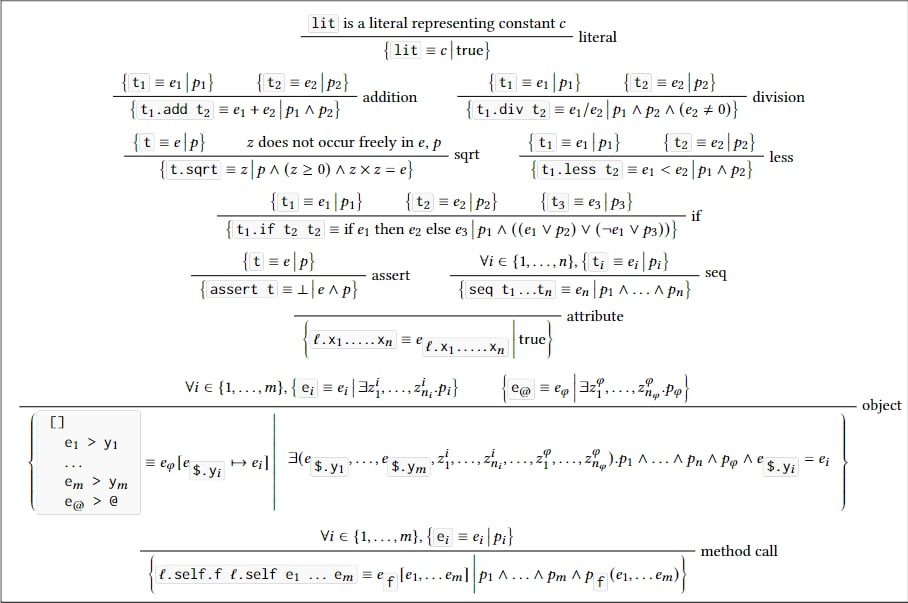
\includegraphics[width=\textwidth]{figs/properties}
  \caption{Rules for property inference in detection of unjustified assumption in subclass.}
  \label{fig:property_inference}
\end{figure}



\subsection{Implementation}
Similarly to the algorithm for the detection of mutual recursion, the tree-like representation of the initial revision of the EO program is done by converting its source code to the \textit{complete object tree} (section \ref{impl:complete_object_tree}). However, in order to produce the revision of the initial program, we needed to implement the inlining procedure for EO syntax tree. This procedure can be summarised as follows:
\begin{enumerate}
  \item Detect all the method calls. This is already done during the construction of the complete object tree.
  \item Replace each method call in the method body with the value of its $\varphi$-attribute (@ symbol in eo).
  \item if the method-object that is inlined contains attributes other than $\varphi$, then:
  \begin{enumerate}
    \item collect these attributes into a separate object called \textit{local\_attrs}. If the attribute with such a name already exists in the object where the call is inlined, resolve the collision by adding a suffix to the newly created object. 
    \item Add this object as a local attribute to the method-object where the call is located. 
    \item Rewire the references to the local attributes inside the $\varphi$ attribute of the methods that is being inlined to their respective attributes in the \textit{local\_attrs} object.
  \end{enumerate}

  \item After the revision of the initial EO code is obtained, the initial object tree and the revised object tree are zipped together in a separate instance of the object tree \pic{fig:zipwithinlined}.

  \item Now that we have all the necessary information about both the initial and revised versions, we need to derive their properties \pic{fig:property_inference}. These properties are encoded as SMTLIB2 \cite{smtlib} programs. We use the \textbf{scala-smtlib} \footnote{\url{https://github.com/regb/scala-smtlib}} library to programmatically construct SMTLIB2-compliant programs. These programs are stored in an auxiliary data structure \ref{fig:property_structure}. This structure has the following fields.
  \item When this structure is constructed for both the initial and revised versions, an implication statement corresponding to the formula \pic{fig:implication} is constructed and passed to the SMT-solver backend. The backend we use in this thesis is called Princess \cite{princess}.
  \item If the solver finds the given to be satisfiable, then there is no error and the revision is considered safe. Otherwise, the revision is considered unsafe and is reported to the user. 
\end{enumerate}

\begin{figure}
\begin{lstlisting}[language=Scala]
  final case class Info(
    forall: List[SortedVar],
    exists: List[SortedVar],
    value: Term,
    properties: Term
  )
\end{lstlisting}
\caption{A data structure for storing the derived properties.}
\label{fig:property_structure}
\end{figure}

\begin{figure}
\begin{lstlisting}[language=Scala]
  final case class MethodInfoForAnalysis(
    selfArgName: String,
    body: EOObj[EOExprOnly],
    depth: Int
  )

  final case class ObjectInfoForAnalysis[P, M](
    methods: Map[EONamedBnd, M],
    parentInfo: Option[P],
    name: Name,
    indirectMethods: Map[
      Name, 
      MethodInfoForAnalysis
    ],
    allMethods: Map[
      Name, 
      MethodInfoForAnalysis
    ]
  )

  type AnalysisInfo = ObjectInfoForAnalysis[
    LinkToParent,
    MethodInfo
  ]
  type InitialAndRevised = ObjectTree[
      (AnalysisInfo, AnalysisInfo)
    ]
\end{lstlisting}
\caption{The object tree used in unjustufied assumption analysis that holds the revised version of the object together with the initial version.}
\label{fig:zipwithinlined}
\end{figure}

\chapter{Evaluation and Discussion}
\label{chap:eval}
This chapter provides the evaluation of the resulting implementation. Section \ref{eval:limitations} outlines the limitations of the EO-based static analysis. Section \ref{eval:testing} describes how the analyzers were tested. Finally, section \ref{eval:comparisons} describes the result of comparing EO-based static analyzers with their counerparts for other programming languages.

\section{Limitations}
\label{eval:limitations}

\subsection{General}
The analyzer provided minimal information about the location of discovered errors. This is especially important if the analyzer is to be used in the integrated development environments.

The analyzer only works on single files. If EO objects are spread across multiple files, the current implementation would be able to analyze only one file at a time. There is a minimal support for objects imported from other EO files, i.e. analyzer acknowledges their existence and does not report them as missing. However, bodies of object imported from other files can not be accessed, therefore no meaningful analysis can be performed if one of the used objects comes from another file.

\subsection{Unanticipated Mutual Recursion}
The implementation of does not do any path-dependent analysis, therefore it may produce false-positives in case when the call to the mutually-recursive method is unreachable, e.g. when guarded by a statement which can only be false.

The current implementation of the mutual recursion analyzer also contains a bug which causes it to crash with a stack overflow exception when the program contains a cycle in the inheritance chains. The presence of the inheritance chain means that there is such a class-object that extends an object which directly or indirectly extends the first object. 

\begin{figure}
  \begin{center}
    \begin{tabular}{c}  
  \lstinputlisting{code/inheritance_chain.eo}
    \end{tabular}
  \end{center}
  \caption{A simple example of the cycle in the inheritance chain as it occurs in EO. Object $a$ extends $b$, which in turn extends object $a$.}
  \label{fig:inheritance_chain}
\end{figure}

\subsection{Unjustified Assumption in Subclass}
The analyzer relies on the external SMT-solver called Princess \cite{princess}. The solver has some limitations when it comes to the support of SMTLIB-2 \cite{smtlib} format. A lot of effort was spent working around the peculiarities of the solver interface. This limits the portability of the implementation if a different SMTLIB backend is to be chosen.

The current implementation of the analyzer supports only a limited set of types. This limitation is directly imposed by the lack of a static type checker in EO. Specifically, all method parameters (excluding \textbf{self}) and their return methods are assumed to be of integer numeric type. This imposes significant limitations on the type of constraints that can be decided by the solver.

Finally, the complexity of the constraints the solver needs to decide grows linearly with the size of the program. While the complexity of the solver operation is largely unknown, it would be safe to estimate that the execution time of the analyzer would be rather slow on the large programs with a lot of constraints.

\section{Testing}
\label{eval:testing}
The implementation is largely covered by hand-written integration tests. The property-based testing technique \cite{property_based_testing} was also applied to the testing of the mutual recursion analyzer to ensure the extensive coverage of the input domain.

\subsection{Integration Testing}
\label{eval:integration_testing}
Integration testing or end-to-end testing \cite[Chapter 7]{testing} describes an approach to testing when one testcase covers the functionality of the entire software system. In our case, the modules under tests where the analyzers, the input was the EO code with or without the respective defects and the expected output was the error messages produced by the respective analyzer, which is represented by a list of strings.

To execute the tests we used a testing framework for Scala called Scalatest \footnote{\url{https://www.scalatest.org/}}. To represent the individual test case we used a the following case class definition:

\begin{lstlisting}[language=Scala]
case class TestCase(
    label: String,
    code: String,
    expected: List[String]
  )
    \end{lstlisting}

The $label$ is a short description of the test case used mostly for human readability. $code$ field holds the code to be analyzed, while the $expected$ field holds the errors that are supposed to be detected by the analyzer in the $code$ field.

All the test cases for a particular analyzer are divided into two groups: one for test cases where the input code contains errors, the other for test cases where the input code does not contain errors. These groups are each represented by a testsuite-local variable of type \textbf{List[TestCase]}:
\begin{lstlisting}[language=Scala]
    val testCasesWithErrors: List[TestCase] = 
        List(casewithErrors1, ..., caseWithErrorsN)
    val testCasesWithoutErrors: List[TestCase] = 
        List(caseWithoutErrors1, ..., caseWithoutErrorsN)
\end{lstlisting}

Each test group is then run using a driver function called $runTests$. This function registers the test in the Scalatest test suite, executes the analyzer on the input code to obtain the errors and then compares the obtained errors with the expected using the assert statement:
\begin{lstlisting}[language=Scala]
    
def runTests(tests: List[TestCase]): Unit =
  tests.foreach { 
    case TestCase(label, code, expected) =>
      registerTest(label) {
        val obtained = analyze(code).unsafeRunSync()
        assert(obtained == expected)
      }
  }

\end{lstlisting}

\subsection{Property-based Testing}
Property-based testing is a variation of random testing that can be used when there exists a set of well-defined properties (or predicates) that should be satisfied for a set of possible inputs of the function being tested.  This predicate is then being evaluated on the randomly generated input data. The key difference between property-based testing and the conventional testing approach, like the one described in \ref{eval:integration_testing}, is the fact that the random input data is generated \textit{automatically}, which covers a large effective subset of the input domain that would otherwise be impractical or impossible to perform manually.

We decided to apply this approach to testing the mutual recursion analyzer as follows:
\begin{enumerate}
  \item 1. Create a generator that randomly generates the instances of \textit{ObjectTreeWithResolvedCallgraphs} \pic{fig:mutualrec_program}. The generation process keeps only those trees that contain the multiobject recursion cycles. These cycles are stored as \textit{CallChain} objects and captured as expected output. 
  \item These trees are converted into string with the respective EO code by a simple pretty-printer.
  \item The analyzer is then run on the generated strings to obtain the \textit{CallChain} objects. The obtained objects are then compared with the ones before pretty-printing. 
\end{enumerate}

So, the property that we are trying to test can be summarised as follows: 

\begin{definition}
  The cycles found in the randomly-generated \textit{ObjectTreeWithResolvedCallgraphs} should be the same as the ones found by the analyzer which was given the pretty-printed version of said \textit{ObjectTreeWithResolvedCallgraphs}.
\end{definition}

The current version of the CI pipeline for the repository runs 1000 such randomly generated tests per run. 

\section{Comparisons}
\label{eval:comparisons}

\chapter{Conclusion}
\label{chap:conclusion}

Nowadays, object-oriented programming paradigm is one of the most dominant tools in the arsenal of software companies. The attempts to keep up with the ever-increasing demand for innovation lead to the inevitable rise in the software complexity. The object-oriented codebases arguably suffered the most from this complexity, giving rise to phenomena such as "legacy code" \cite{legacy}. There are many existing approaches for taming this complexity. One of the most commonly used is called static analysis - reasoning about the code without executing it. 

This thesis described an innovative approach to the static analysis of object-oriented programs involving $\varphi$-calculus - a formalization of the object-oriented semantics based on the idea of the decorator pattern \cite{GOFPatterns}. We studied the existing works on $\varphi$-calculus and its implementation, EO \cite{eolang}, described one of the variations of $\varphi$-calculus and applied it to building a static analyzer that detects the problems of the "fragile base class" \cite{fragilebaseclass} family. The implementation was documented and the source code  was published to an open source Github repository.

The analyzer has been extensively tested using hand-written examples. There are currently 89 tests being run in the continuous integration pipeline, some of them approaching 700 lines of EO code. 

\section{Contribution Summary}
\begin{itemize}
    \item A parser for a subset of EO grammar described in \cite{eolang}.
    \item A set of useful data structures for analyzing the programs translated to the EO intermediate representation. 
    \item Two algorithms that use the above data structures to detect two defects of the "fragile base class" family - unanticipated mutual recursion and unjustified assumption in subclass.
\end{itemize}

\section{Future Work}
A significant body of work was done, however there are still problems to be solved before the analyzers that use the approach described in this thesis can find defects in industrial-scale object-oriented codebases. 

\begin{itemize}
    \item The analyzers described in this thesis need to be coupled with a translator from the target language (e.g. Java) to the EO intermediate representation. We are aware of several of several existing works in this area, however little work was done to make them work together with the analyzers.
    \item Performing complicated analyses such as detecting of unjustified assumption in subclass is significantly crippled by the lack of type checker in EO. Having information about the object types during the analysis would make the process of constraint inference such as the one described in \ref{impl:unjustified_algo} more robust and precise. 
    \item The analyzers run successfully on small test cases, however testing them on bigger bodies of EO code, e.g. generated from the existing Java source code, may reveal critical flaws in the current design, as well as the performance bottlenecks that are hard to detect on smaller test cases. 
    \item The current design of the analyzers does not take into account the error reporting, so its current capabilities are limited to fully-qualified names of the objects where the errors occurred. The design needs to be revised to make error messages point to the exact locations of errors in the EO intermediate representation and conseqiently in the target language source code.
\end{itemize}




%% REFERENCES
% \printbibliography[heading=bibintoc,title={Bibliography cited}]
% \appendix
\chapter{Extra Stuff}
\blindtext

\chapter{Even More Extra Stuff}
\blindtext
\end{document}

